\PassOptionsToPackage{unicode=true}{hyperref} % options for packages loaded elsewhere
\PassOptionsToPackage{hyphens}{url}
%
\documentclass[10pt,xcolor=table,color={dvipsnames,usenames},ignorenonframetext,usepdftitle=false,french,aspectratio=169]{beamer}
\setbeamertemplate{caption}[numbered]
\setbeamertemplate{caption label separator}{: }
\setbeamercolor{caption name}{fg=normal text.fg}
\beamertemplatenavigationsymbolsempty
\usepackage{caption}
\captionsetup{skip=0pt,belowskip=0pt}
%\setlength\abovecaptionskip{-15pt}
\usepackage{lmodern}
\usepackage{amssymb,amsmath,mathtools,multirow}
\usepackage{float,hhline}
\usepackage{tikz}
\usepackage{mathtools}
\usepackage{ifxetex,ifluatex}
\usepackage{fixltx2e} % provides \textsubscript
\ifnum 0\ifxetex 1\fi\ifluatex 1\fi=0 % if pdftex
  \usepackage[T1]{fontenc}
  \usepackage[utf8]{inputenc}
  \usepackage{textcomp} % provides euro and other symbols
\else % if luatex or xelatex
  \usepackage{unicode-math}
  \defaultfontfeatures{Ligatures=TeX,Scale=MatchLowercase}
\fi
\usetheme[coding=utf8,language=english,
,titlepagelogo=img/SACElogo
]{TorinoTh}
% use upquote if available, for straight quotes in verbatim environments
\IfFileExists{upquote.sty}{\usepackage{upquote}}{}
% use microtype if available
\IfFileExists{microtype.sty}{%
\usepackage[]{microtype}
\UseMicrotypeSet[protrusion]{basicmath} % disable protrusion for tt fonts
}{}
\IfFileExists{parskip.sty}{%
\usepackage{parskip}
}{% else
\setlength{\parindent}{0pt}
\setlength{\parskip}{6pt plus 2pt minus 1pt}
}
\usepackage{hyperref}
\hypersetup{
            pdfauthor={Anna Smyk and Tanguy Barthelemy},
            pdfborder={0 0 0},
            breaklinks=true}
\urlstyle{same}  % don't use monospace font for urls
\newif\ifbibliography
\newlength{\cslhangindent}
\setlength{\cslhangindent}{1.5em}
\newlength{\csllabelwidth}
\setlength{\csllabelwidth}{3em}
\newenvironment{CSLReferences}[2] % #1 hanging-ident, #2 entry spacing
 {% don't indent paragraphs
  \setlength{\parindent}{0pt}
  % turn on hanging indent if param 1 is 1
  \ifodd #1 \everypar{\setlength{\hangindent}{\cslhangindent}}\ignorespaces\fi
  % set entry spacing
  \ifnum #2 > 0
  \setlength{\parskip}{#2\baselineskip}
  \fi
 }%
 {}
\usepackage{color}
\usepackage{fancyvrb}
\newcommand{\VerbBar}{|}
\newcommand{\VERB}{\Verb[commandchars=\\\{\}]}
\DefineVerbatimEnvironment{Highlighting}{Verbatim}{commandchars=\\\{\}}
% Add ',fontsize=\small' for more characters per line
\usepackage{framed}
\definecolor{shadecolor}{RGB}{248,248,248}
\newenvironment{Shaded}{\begin{snugshade}}{\end{snugshade}}
\newcommand{\AlertTok}[1]{\textcolor[rgb]{0.94,0.16,0.16}{#1}}
\newcommand{\AnnotationTok}[1]{\textcolor[rgb]{0.56,0.35,0.01}{\textbf{\textit{#1}}}}
\newcommand{\AttributeTok}[1]{\textcolor[rgb]{0.77,0.63,0.00}{#1}}
\newcommand{\BaseNTok}[1]{\textcolor[rgb]{0.00,0.00,0.81}{#1}}
\newcommand{\BuiltInTok}[1]{#1}
\newcommand{\CharTok}[1]{\textcolor[rgb]{0.31,0.60,0.02}{#1}}
\newcommand{\CommentTok}[1]{\textcolor[rgb]{0.56,0.35,0.01}{\textit{#1}}}
\newcommand{\CommentVarTok}[1]{\textcolor[rgb]{0.56,0.35,0.01}{\textbf{\textit{#1}}}}
\newcommand{\ConstantTok}[1]{\textcolor[rgb]{0.00,0.00,0.00}{#1}}
\newcommand{\ControlFlowTok}[1]{\textcolor[rgb]{0.13,0.29,0.53}{\textbf{#1}}}
\newcommand{\DataTypeTok}[1]{\textcolor[rgb]{0.13,0.29,0.53}{#1}}
\newcommand{\DecValTok}[1]{\textcolor[rgb]{0.00,0.00,0.81}{#1}}
\newcommand{\DocumentationTok}[1]{\textcolor[rgb]{0.56,0.35,0.01}{\textbf{\textit{#1}}}}
\newcommand{\ErrorTok}[1]{\textcolor[rgb]{0.64,0.00,0.00}{\textbf{#1}}}
\newcommand{\ExtensionTok}[1]{#1}
\newcommand{\FloatTok}[1]{\textcolor[rgb]{0.00,0.00,0.81}{#1}}
\newcommand{\FunctionTok}[1]{\textcolor[rgb]{0.00,0.00,0.00}{#1}}
\newcommand{\ImportTok}[1]{#1}
\newcommand{\InformationTok}[1]{\textcolor[rgb]{0.56,0.35,0.01}{\textbf{\textit{#1}}}}
\newcommand{\KeywordTok}[1]{\textcolor[rgb]{0.13,0.29,0.53}{\textbf{#1}}}
\newcommand{\NormalTok}[1]{#1}
\newcommand{\OperatorTok}[1]{\textcolor[rgb]{0.81,0.36,0.00}{\textbf{#1}}}
\newcommand{\OtherTok}[1]{\textcolor[rgb]{0.56,0.35,0.01}{#1}}
\newcommand{\PreprocessorTok}[1]{\textcolor[rgb]{0.56,0.35,0.01}{\textit{#1}}}
\newcommand{\RegionMarkerTok}[1]{#1}
\newcommand{\SpecialCharTok}[1]{\textcolor[rgb]{0.00,0.00,0.00}{#1}}
\newcommand{\SpecialStringTok}[1]{\textcolor[rgb]{0.31,0.60,0.02}{#1}}
\newcommand{\StringTok}[1]{\textcolor[rgb]{0.31,0.60,0.02}{#1}}
\newcommand{\VariableTok}[1]{\textcolor[rgb]{0.00,0.00,0.00}{#1}}
\newcommand{\VerbatimStringTok}[1]{\textcolor[rgb]{0.31,0.60,0.02}{#1}}
\newcommand{\WarningTok}[1]{\textcolor[rgb]{0.56,0.35,0.01}{\textbf{\textit{#1}}}}
\usepackage{graphicx,grffile}
\makeatletter
\def\maxwidth{\ifdim\Gin@nat@width>\linewidth\linewidth\else\Gin@nat@width\fi}
\def\maxheight{\ifdim\Gin@nat@height>\textheight\textheight\else\Gin@nat@height\fi}
\makeatother
% Scale images if necessary, so that they will not overflow the page
% margins by default, and it is still possible to overwrite the defaults
% using explicit options in \includegraphics[width, height, ...]{}
\setkeys{Gin}{width=\maxwidth,height=\maxheight,keepaspectratio}
% Prevent slide breaks in the middle of a paragraph:
\widowpenalties 1 10000
\raggedbottom
\AtBeginPart{
  \let\insertpartnumber\relax
  \let\partname\relax
  \frame{\partpage}
}
\AtBeginSection{
  \ifbibliography
  \else
    \begin{frame}[noframenumbering]{Contents}
    \tableofcontents[currentsection, hideothersubsections]
    \end{frame}
  \fi
}
\setlength{\emergencystretch}{3em}  % prevent overfull lines
\providecommand{\tightlist}{%
  %\setlength{\itemsep}{0pt}
  \setlength{\parskip}{0pt}
  }
\setcounter{secnumdepth}{0}

% set default figure placement to htbp
\makeatletter
\def\fps@figure{htbp}
\makeatother

\usepackage{dsfont}
\usepackage{stmaryrd}
\usepackage[normalem]{ulem}
\usepackage{fontawesome5}
\usepackage{tikz,pgfplots}
\pgfplotsset{compat=1.17}
\pgfplotsset{samples=100}
\usepackage{animate}
 \usepackage{booktabs}

\usepackage{colortbl}

\DeclareMathOperator{\Cov}{Cov}
\newcommand{\cov}[2]{\Cov\left( #1\,,\,#2 \right)}

\DeclareMathOperator{\e}{e}
\renewcommand{\P}{\mathds{P}} %Apparement \P existe déjà ?
\newcommand\N{\mathds{N}}
\newcommand\R{\mathds{R}}


\newcommand\1{\mathds{1}}
\newcommand{\E}[2][]{{\mathds{E}}_{#1}
  \def\temp{#2}\ifx\temp\empty
  \else
    \left[#2\right]
  \fi
}
\newcommand{\V}[2][]{{\mathds{V}}_{#1}
  \def\temp{#2}\ifx\temp\empty
  \else
    \left[#2\right]
  \fi
}
\newcommand\ud{\,\mathrm{d}}


% blocks
\usepackage{environ}
\usepackage[tikz]{bclogo}

\tikzstyle{titlestyle} =[draw=black!80,fill=black!20, text=black,
 right=10pt, rounded corners]
\mdfdefinestyle{symmaryboxstyle}{
	linecolor=black!80, backgroundcolor = black!5,
	skipabove=\baselineskip, innertopmargin=\baselineskip,
	innerbottommargin=\baselineskip,
	userdefinedwidth=\textwidth,
	middlelinewidth=1.2pt, roundcorner=5pt,
	skipabove={\dimexpr0.5\baselineskip+\topskip\relax},
	frametitleaboveskip=\dimexpr-\ht\strutbox\relax,
	innerlinewidth=0pt,
}
\NewEnviron{summary}{%
\begin{mdframed}[style=symmaryboxstyle]
\vspace{-0.5em}
\BODY
\end{mdframed}
}
\makeatletter
% Open `\noalign` and check for overlay specification:
\def\rowcolor{\noalign{\ifnum0=`}\fi\bmr@rowcolor}
\newcommand<>{\bmr@rowcolor}{%
    \alt#1%
        {\global\let\CT@do@color\CT@@do@color\@ifnextchar[\CT@rowa\CT@rowb}% Rest of original `\rowcolor`
        {\ifnum0=`{\fi}\@gooble@rowcolor}% End `\noalign` and gobble all arguments of `\rowcolor`.
}
% Gobble all normal arguments of `\rowcolor`:
\newcommand{\@gooble@rowcolor}[2][]{\@gooble@rowcolor@}
\newcommand{\@gooble@rowcolor@}[1][]{\@gooble@rowcolor@@}
\newcommand{\@gooble@rowcolor@@}[1][]{\ignorespaces}

\newcommand{\rowc}[1]{\only<#1>{\\\rowcolor{processblue!40}}}
%\newcommand{\rowc}[1]{{\rowcolor<#1>{processblue!30}}
\newcommand{\cellc}[1]{\only<#1>{\cellcolor{processblue!40}}}
\newcommand{\supsp}[1]{\visible<#1>{\\}}

\title{Using JDemetra+ in R: from version 2 to version 3\\
Presentation 3: Wrangling workspaces in R}
\ateneo{TSACE Webinar, Wednesday December 14th 2022}
\author{Anna Smyk and Tanguy Barthelemy}
\date{}


\setrellabel{}

\setcandidatelabel{}

\rel{}
\division{With the collaboration of Alain Quartier-la-tente\\}

\departement{}
\makeatletter
\let\@@magyar@captionfix\relax
\makeatother


\begin{document}
\begin{frame}[plain,noframenumbering]
\titlepage
\end{frame}

\hypertarget{introduction}{%
\section{Introduction}\label{introduction}}

\hypertarget{context}{%
\subsection{Context}\label{context}}

\begin{frame}{Context}
\begin{itemize}
\item
  in R we don't need a workspace stucture to run an SA process (cf P2)
\item
  we could think SA processing with JD+ algorithms can happen in two
  distinct worlds

  \begin{itemize}
  \tightlist
  \item
    graphical user interface (GUI) and cruncher using workspaces
  \end{itemize}

  OR

  \begin{itemize}
  \tightlist
  \item
    R functions (without workpaces, TS object or numeric vectors for HF)
  \end{itemize}
\end{itemize}

Still there are benefits in using workspaces and R packages in
conjunction

We will highlight them in the remaining of this presentation
\end{frame}

\begin{frame}{Workspace structure}
\protect\hypertarget{workspace-structure}{}
\begin{itemize}
\tightlist
\item
  a workspace is a JD+ specific data structure (XML files) which allows
  to use the GUI and cruncher
\end{itemize}

Workspaces have two diserable properties:

\begin{itemize}
\tightlist
\item
  reading by GUI (1)
\item
  refreshing (with new raw data for example) by GUI or cruncher (2)
\end{itemize}

If a workspace doesn't contain the sufficient metadata (path to the raw
data), only the first property (1) will be available.
\end{frame}

\begin{frame}{SA-item in XML files}
\protect\hypertarget{sa-item-in-xml-files}{}
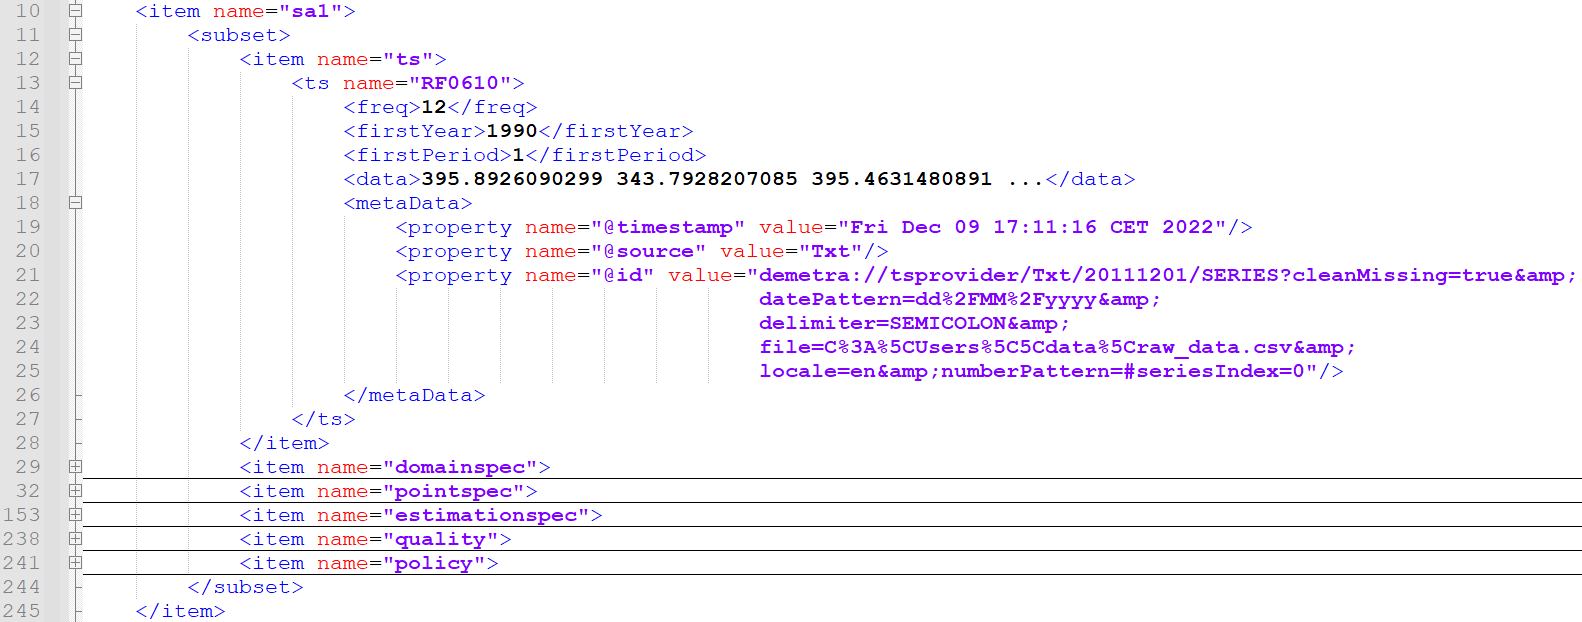
\includegraphics{img/SA-item-XML.PNG}
\end{frame}

\hypertarget{using-workspaces-and-r-packages-in-conjuction}{%
\section{Using workspaces and R packages in
conjuction}\label{using-workspaces-and-r-packages-in-conjuction}}

\begin{frame}{Using workspaces and R packages in conjuction}
\protect\hypertarget{using-workspaces-and-r-packages-in-conjuction-1}{}
Two principal classes of benefits:

\begin{itemize}
\tightlist
\item
  instant reading: immersing results in the R world (functions, plots..)
\item
  automating potential manual operations for large datasets
\end{itemize}
\end{frame}

\begin{frame}[fragile]{Packages operating on workspaces}
\protect\hypertarget{packages-operating-on-workspaces}{}
We will use the packages
\href{https://github.com/jdemetra/rjdemetra}{\textbf{RJDemetra}},
\href{https://github.com/palatej/rjdemetra3}{\textbf{rjdemetra3}} and
\href{https://github.com/InseeFrLab/rjdworkspace}{\textbf{rjdworkspace}}.

The packages are availiable here:

\begin{itemize}
\tightlist
\item
  \href{https://github.com/jdemetra/rjdemetra}{\textbf{RJDemetra}} on
  \href{https://cran.r-project.org/web/packages/RJDemetra/index.html}{CRAN}
  or \url{https://github.com/jdemetra/rjdemetra}
\item
  \href{https://github.com/palatej/rjdemetra3}{\textbf{rjdemetra3}} on
  \url{https://github.com/palatej/rjdemetra3}
\item
  \href{https://github.com/InseeFrLab/rjdworkspace}{\textbf{rjdworkspace}}
  on \url{https://github.com/InseeFrLab/rjdworkspace}.
\end{itemize}

To install it use the following code:

\footnotesize

\begin{Shaded}
\begin{Highlighting}[]
\CommentTok{\# If devtools is not installed}
\CommentTok{\# install.packages("devtools")}
\FunctionTok{library}\NormalTok{(}\StringTok{"devtools"}\NormalTok{)}

\FunctionTok{install.packages}\NormalTok{(}\StringTok{"RJDemetra"}\NormalTok{)}
\FunctionTok{install\_github}\NormalTok{(}\StringTok{"https://github.com/palatej/rjdemetra3"}\NormalTok{)}
\FunctionTok{install\_github}\NormalTok{(}\StringTok{"https://github.com/InseeFrLab/rjdworkspace"}\NormalTok{)}
\end{Highlighting}
\end{Shaded}
\end{frame}

\hypertarget{instant-reading}{%
\section{Instant reading}\label{instant-reading}}

\begin{frame}{Instant reading of workspaces}
\protect\hypertarget{instant-reading-of-workspaces}{}
In a workspace, we read:

\begin{itemize}
\tightlist
\item
  output series
\item
  parameters
\item
  diagnostics
\end{itemize}

Thanks to R packages, no export + import but directly:

\begin{itemize}
\tightlist
\item
  import in R physical workspaces
\item
  automatic and chain reading --\textgreater{} many series and quickly
\item
  make faster comparisons
\end{itemize}
\end{frame}

\begin{frame}[fragile]{Instant reading in v2}
\protect\hypertarget{instant-reading-in-v2}{}
In \href{https://github.com/jdemetra/rjdemetra}{\textbf{RJDemetra}}
(v2), the function \texttt{RJDemetra::load\_workspace()} creates a
connection between a physical workspace and a R object and allows to
read every multiprocessing and SA-items.

Code example:

\footnotesize

\begin{Shaded}
\begin{Highlighting}[]
\NormalTok{ws }\OtherTok{\textless{}{-}}\NormalTok{ RJDemetra}\SpecialCharTok{::}\FunctionTok{load\_workspace}\NormalTok{(}\StringTok{"./WS\_input/WS\_simple.xml"}\NormalTok{)}
\NormalTok{RJDemetra}\SpecialCharTok{::}\FunctionTok{compute}\NormalTok{(ws)}

\NormalTok{mp\_1 }\OtherTok{\textless{}{-}}\NormalTok{ RJDemetra}\SpecialCharTok{::}\FunctionTok{get\_object}\NormalTok{(ws, }\AttributeTok{pos =} \DecValTok{1}\NormalTok{)}
\NormalTok{sa\_item\_1 }\OtherTok{\textless{}{-}}\NormalTok{ RJDemetra}\SpecialCharTok{::}\FunctionTok{get\_object}\NormalTok{(mp\_1, }\AttributeTok{pos =} \DecValTok{1}\NormalTok{)}
\NormalTok{model\_sa\_1 }\OtherTok{\textless{}{-}}\NormalTok{ RJDemetra}\SpecialCharTok{::}\FunctionTok{get\_model}\NormalTok{(sa\_item\_1, }\AttributeTok{workspace =}\NormalTok{ ws)}
\end{Highlighting}
\end{Shaded}

\normalsize

Later we will produce the same workspace result with
\href{https://github.com/jdemetra/rjdemetra}{\textbf{RJDemetra}} in the
\textbf{\protect\hyperlink{reproduce-workspace}{Reproduce workspace}}
section.
\end{frame}

\begin{frame}[fragile]{Instant reading in v3}
\protect\hypertarget{instant-reading-in-v3}{}
In \href{https://github.com/palatej/rjdemetra3}{\textbf{rjdemetra3}}
(v3), the function \texttt{rjdemetra3::load\_workspace} imports directly
in our R working directory all the informations (multiprocessing,
SA-item\ldots) in a R object (list).

Code example:

\footnotesize

\begin{Shaded}
\begin{Highlighting}[]
\NormalTok{ws }\OtherTok{\textless{}{-}}\NormalTok{ rjdemetra3}\SpecialCharTok{::}\FunctionTok{load\_workspace}\NormalTok{(}\StringTok{"./WS\_input/WS\_simple.xml"}\NormalTok{)}
\end{Highlighting}
\end{Shaded}

\normalsize

This single line does the same job as the previous 5 of version 2.

Today, the connection between R packages v3 and the workspace structure
is under construction.

There are no functions yet to navigate this object. So from now on, I
will only present the functions of version 2.
\end{frame}

\hypertarget{automating-operations}{%
\section{Automating operations}\label{automating-operations}}

\begin{frame}{Automating operations on workspaces}
\protect\hypertarget{automating-operations-on-workspaces}{}
Goals:

\begin{itemize}
\tightlist
\item
  produce and reproduce the workspace structure without the JDemetra+
  GUI but with R
\item
  keep the reading, writing and refreshing properties both by the GUI
  and by the cruncher
\item
  enable dynamic updates of physical workspaces with R
\end{itemize}
\end{frame}

\begin{frame}{Outline of the automation}
\protect\hypertarget{outline-of-the-automation}{}
Different kind of operations possible in R:

\begin{itemize}
\tightlist
\item
  creation of workspaces, multiprocessing and SA-item
\item
  export and write a workspace (physical XML files)
\item
  modification / dynamic update with one or several workspaces
\end{itemize}
\end{frame}

\hypertarget{creation}{%
\subsection{Creation}\label{creation}}

\begin{frame}[fragile]{Creation of a workspace}
\protect\hypertarget{creation-of-a-workspace}{}
\href{https://github.com/jdemetra/rjdemetra}{\textbf{RJDemetra}} has a
collection of functions to create a workspace and each element
(multiprocessing, SA-item\ldots) and to bring it together:

\begin{itemize}
\tightlist
\item
  create a \emph{virtual} workspace:
  \texttt{RJDemetra::new\_workspace()}
\item
  create a \emph{virtual} multiprocessing:
  \texttt{RJDemetra::new\_multiprocessing()}
\item
  create a specification, there are several functions depending on the
  method:
  \texttt{RJDemetra::x13\_spec(),\ RJDemetra::tramoseats\_spec()...}
\item
  create an SA-item, there are several functions depending on the chosen
  specification: \texttt{RJDemetra::x13(),\ RJDemetra::tramoseats()...}
\item
  Finally to bring the elements together, you can use
  \texttt{RJDemetra::add\_sa\_item()} to add the created SA-item to a
  multprocessing in your workspace
\end{itemize}

\emph{virtual object = composed of R object}
\end{frame}

\begin{frame}[fragile]{Reproduce workspace}
\protect\hypertarget{reproduce-workspace}{}
Here we reproduce the SA-item read in the
\textbf{\protect\hyperlink{instant-reading-in-v2}{Instant reading in
v2}} section

\footnotesize

\begin{Shaded}
\begin{Highlighting}[]
\CommentTok{\# Data preparation}
\NormalTok{raw\_data }\OtherTok{\textless{}{-}} \FunctionTok{read.csv2}\NormalTok{(}\StringTok{"./data/raw\_data.csv"}\NormalTok{, }\AttributeTok{dec =} \StringTok{"."}\NormalTok{) }\SpecialCharTok{|\textgreater{}} 
    \FunctionTok{ts}\NormalTok{(}\AttributeTok{start =} \DecValTok{1990}\NormalTok{, }\AttributeTok{frequency =} \DecValTok{12}\NormalTok{)}

\CommentTok{\# Create WS}
\NormalTok{ws }\OtherTok{\textless{}{-}}\NormalTok{ RJDemetra}\SpecialCharTok{::}\FunctionTok{new\_workspace}\NormalTok{()}
\NormalTok{mp\_1 }\OtherTok{\textless{}{-}}\NormalTok{ RJDemetra}\SpecialCharTok{::}\FunctionTok{new\_multiprocessing}\NormalTok{(}\AttributeTok{workspace =}\NormalTok{ ws, }
                                       \AttributeTok{name =} \StringTok{"SAProcessing{-}1"}\NormalTok{)}
\NormalTok{spec\_x13 }\OtherTok{\textless{}{-}}\NormalTok{ RJDemetra}\SpecialCharTok{::}\FunctionTok{x13\_spec}\NormalTok{(}\AttributeTok{spec =} \StringTok{"RSA3"}\NormalTok{)}
\NormalTok{model\_sa\_1 }\OtherTok{\textless{}{-}}\NormalTok{ RJDemetra}\SpecialCharTok{::}\FunctionTok{x13}\NormalTok{(raw\_data, }\AttributeTok{spec =}\NormalTok{ spec\_x13)}
\end{Highlighting}
\end{Shaded}
\end{frame}

\hypertarget{export}{%
\subsection{Export}\label{export}}

\begin{frame}[fragile]{Export}
For the export part, the function \texttt{RJDemetra::save\_workspace()}
exports and creates a workspace (XML files).

Warning: if the workspace has been created by
\texttt{RJDemetra::new\_workspace()}, he won't contain sufficient
metadata to be refreshable by the GUI or the cruncher.
\end{frame}

\begin{frame}{\href{https://github.com/InseeFrLab/rjdworkspace}{\textbf{rjdworkspace}}
and dynamic update}
\protect\hypertarget{rjdworkspace-and-dynamic-update}{}
\href{https://github.com/InseeFrLab/rjdworkspace}{\textbf{rjdworkspace}}
is a package developed by \href{https://github.com/InseeFrLab}{Insee} to
fill in the gaps between the workspace structure and R.

It relies on
\href{https://github.com/jdemetra/rjdemetra}{\textbf{RJDemetra}} (v2)
but will be soon added to the new package
\href{https://github.com/palatej/rjdemetra3}{\textbf{rjdemetra3}}.
\href{https://github.com/InseeFrLab/rjdworkspace}{\textbf{rjdworkspace}}
only works with physical workspaces (XML files).
\end{frame}

\begin{frame}{\href{https://github.com/InseeFrLab/rjdworkspace}{\textbf{rjdworkspace}}
features}
\protect\hypertarget{rjdworkspace-features}{}
The features offered by this package are:

\begin{itemize}
\tightlist
\item
  Modification on 1 workspace:

  \begin{itemize}
  \tightlist
  \item
    handle SA-object
  \item
    handle metadata
  \end{itemize}
\item
  Modification on 2 workspaces:

  \begin{itemize}
  \tightlist
  \item
    update a workspace with the informations contained in another one
  \item
    transfert SA-object from a workspace to another
  \end{itemize}
\end{itemize}

\emph{SA-object = \{SA-item, multiprocessing\ldots\}}

\href{https://github.com/InseeFrLab/rjdworkspace}{\textbf{rjdworkspace}}
operations always keep workspaces readable by GUI and refreshable with
the GUI and the cruncher.
\end{frame}

\hypertarget{handling-sa-item}{%
\subsection{Handling SA-item}\label{handling-sa-item}}

\begin{frame}[fragile]{Handling SA-item}
To handle SA-item, it is possible to:

\begin{itemize}
\tightlist
\item
  add new SA-item: \texttt{rjdworkspace::add\_new\_sa\_item()}
\item
  remove a SA-item: \texttt{rjdworkspace::remove\_sa\_item()}
\item
  replace a SA-item by another:
  \texttt{rjdworkspace::replace\_sa\_item()}
\item
  modify a SA-item: \texttt{rjdworkspace::set\_name()},
  \texttt{rjdworkspace::set\_spec()} and
  \texttt{rjdworkspace::set\_ts()}
\end{itemize}
\end{frame}

\begin{frame}[fragile]{Handling metadata}
\protect\hypertarget{handling-metadata}{}
\begin{itemize}
\item
  handling comments: \texttt{rjdworkspace::get\_comment()} and
  \texttt{rjdworkspace::set\_comment()}
\item
  handling raw data path: \texttt{rjdworkspace::update\_path()}
\end{itemize}
\end{frame}

\hypertarget{handling-several-workspaces}{%
\subsection{Handling several
workspaces}\label{handling-several-workspaces}}

\begin{frame}[fragile]{Handling several workspaces}
\begin{itemize}
\item
  update SA-item: \texttt{rjdworkspace::replace\_series()},
  \texttt{rjdworkspace::transfer\_series()}
\item
  handling all metadata: \texttt{rjdworkspace::update\_metadata()}
\end{itemize}
\end{frame}

\hypertarget{conclusion}{%
\section{Conclusion}\label{conclusion}}

\begin{frame}{Summary of available functionalities}
\protect\hypertarget{summary-of-available-functionalities}{}
With the combination of
\href{https://github.com/jdemetra/rjdemetra}{\textbf{RJDemetra}} and
\href{https://github.com/InseeFrLab/rjdworkspace}{\textbf{rjdworkspace}},
there are a lot of features to handle workspaces with R.

In an annual review, it makes it easier to:

\begin{itemize}
\tightlist
\item
  copy, merge and update workspaces
\item
  update and select SA-item
\end{itemize}

than doing it by hand with the GUI.
\end{frame}

\begin{frame}{Missing functionalities and future developement}
\protect\hypertarget{missing-functionalities-and-future-developement}{}
Unfortunately, the creation of workspace is not totally elaborated and
developped. The current version using RJDemetra can't create workspaces
which are readable and refreshable by the GUI from scratch.

The version 3 is under construction. In the future, it will contain the
functions of
\href{https://github.com/InseeFrLab/rjdworkspace}{\textbf{rjdworkspace}}
and will be further expanded.
\end{frame}

\end{document}
